\appendix
	\chapter{IEEE 33 BUS SYSTEM}
%\flushleft
This test system and its data are referred from \cite{rao}. In base case (i.e) topology I, there are five open tie switches and branch numbers are 33, 34, 35, 36, and 37 respectively. In topology II, the five open tie switches and branch numbers are 7, 9, 14, 32, and 37 respectively.  The single line diagram of the IEEE 33 bus system is shown in Fig. \ref{fig:single33}. The total real and reactive power loads on the system are 3715 $kW$ and 2300 $kVAr$ respectively. The voltage magnitude of the system is 1\angle\ang{0} p.u.

\begin{figure}[ht]
		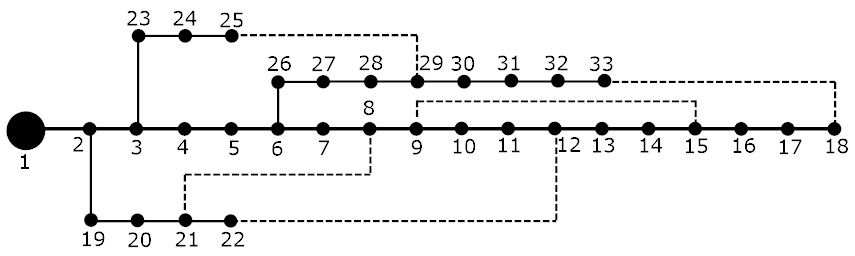
\includegraphics[width=1\textwidth]{./Figures/33bus_singleline_diagram_tieline_t1}
	\caption{Single line diagram of IEEE-33 Bus System}
	\label{fig:single33}
\end{figure}

\pagebreak
	\begin{longtable}{cccccccccc}
		\caption {IEEE 33 Bus System Bus Data}
		\label{table:busdata33}
		\hline
		\multirow{1}{*}{\begin{tabular}[c]{@{}c@{}}Bus \\ No.\end{tabular}} & \multirow{1}{*}{\begin{tabular}[c]{@{}c@{}}Bus \\ Code\end{tabular}} & \multirow{1}{*}{\begin{tabular}[c]{@{}c@{}}Load\\ Type\end{tabular}} & \multicolumn{2}{c}{Load} & \multicolumn{4}{c}{Generator} & \multirow{1}{*}{\begin{tabular}[c]{@{}c@{}}Injected \\ MVAr\end{tabular}} \\
		\cmidrule{4-5} 
		\cmidrule(lr{1em}){6-9}
		&  &  & \multirow{1}{*}{MW} & \multirow{1}{*}{MVAr} & \multirow{1}{*}{MW} & \multirow{1}{*}{MVAr} & \multirow{1}{*}{Qmin} & \multirow{1}{*}{Qmax} &  \\
		&  &  &  &  &  &  &  &  &  \\
		\cmidrule(lr){1-10}
		1 & 1 & -           & 0     & 0     & 0 & 0 & 0 & 0 & 0 \\
		2 & 0 & Curtailable & 0.100 & 0.060 & 0 & 0 & 0 & 0 & 0 \\
		3 & 0 & Curtailable & 0.090 & 0.040 & 0 & 0 & 0 & 0 & 0 \\
		4 & 0 & Curtailable & 0.120 & 0.080 & 0 & 0 & 0 & 0 & 0 \\
		5 & 0 & Curtailable & 0.060 & 0.030 & 0 & 0 & 0 & 0 & 0 \\
		6 & 0 & Fixed & 0.060 & 0.020 & 0 & 0 & 0 & 0 & 0 \\
		7 & 0 & Fixed & 0.200 & 0.100 & 0 & 0 & 0 & 0 & 0 \\
		8 & 0 & Fixed & 0.200 & 0.100 & 0 & 0 & 0 & 0 & 0 \\
		9 & 0 & Fixed & 0.060 & 0.020 & 0 & 0 & 0 & 0 & 0 \\
		10 & 0 & Fixed & 0.060 & 0.020 & 0 & 0 & 0 & 0 & 0 \\
		11 & 0 & Fixed & 0.045 & 0.020 & 0 & 0 & 0 & 0 & 0 \\
		12 & 0 & Controllable & 0.060 & 0.035 & 0 & 0 & 0 & 0 & 0 \\
		13 & 0 & Controllable & 0.060 & 0.035 & 0 & 0 & 0 & 0 & 0 \\
		14 & 0 & Controllable & 0.120 & 0.080 & 0 & 0 & 0 & 0 & 0 \\
		15 & 0 & Controllable & 0.060 & 0.010 & 0 & 0 & 0 & 0 & 0 \\
		16 & 0 & Controllable & 0.060 & 0.020 & 0 & 0 & 0 & 0 & 0 \\
		17 & 0 & Controllable & 0.060 & 0.020 & 0 & 0 & 0 & 0 & 0 \\
		18 & 0 & Controllable & 0.090 & 0.040 & 0 & 0 & 0 & 0 & 0 \\
		19 & 0 & Controllable & 0.090 & 0.040 & 0 & 0 & 0 & 0 & 0 \\
		20 & 0 & Controllable & 0.090 & 0.040 & 0 & 0 & 0 & 0 & 0 \\
		21 & 0 & Controllable & 0.090 & 0.040 & 0 & 0 & 0 & 0 & 0 \\
		22 & 0 & Controllable & 0.090 & 0.040 & 0 & 0 & 0 & 0 & 0 \\
		23 & 0 & Controllable & 0.090 & 0.050 & 0 & 0 & 0 & 0 & 0 \\
		24 & 0 & Controllable & 0.420 & 0.200 & 0 & 0 & 0 & 0 & 0 \\
		25 & 0 & Controllable & 0.420 & 0.200 & 0 & 0 & 0 & 0 & 0 \\
		26 & 0 & Curtailable & 0.060 & 0.025 & 0 & 0 & 0 & 0 & 0 \\
		27 & 0 & Curtailable & 0.060 & 0.025 & 0 & 0 & 0 & 0 & 0 \\
		28 & 0 & Curtailable & 0.060 & 0.020 & 0 & 0 & 0 & 0 & 0 \\
		29 & 0 & Curtailable & 0.120 & 0.070 & 0 & 0 & 0 & 0 & 0 \\
		30 & 0 & Curtailable & 0.200 & 0.600 & 0 & 0 & 0 & 0 & 0 \\
		31 & 0 & Curtailable & 0.150 & 0.070 & 0 & 0 & 0 & 0 & 0 \\
		32 & 0 & Curtailable & 0.210 & 0.100 & 0 & 0 & 0 & 0 & 0 \\
		33 & 0 & Curtailable & 0.060 & 0.040 & 0 & 0 & 0 & 0 & 0 \\
	\bottomrule %[1.5pt]		
\end{longtable}
\begin{flushleft}
	%\flushleft
	\item  Bus Code
	\newline 1 - Slack Bus \newline 0 - Load Bus
	
\end{flushleft}	

	\begin{longtable}{ccccccccc}
	\caption {IEEE 33 Bus System Line Data}
	\label{table:linedata33}
	\hline
	\multirow{4}{*}{\begin{tabular}[c]{@{}c@{}}  Line \\ No.\end{tabular}} & \multirow{4}{*}{\begin{tabular}[c]{@{}c@{}}From\\ Bus\end{tabular}} & \multirow{4}{*}{\begin{tabular}[c]{@{}c@{}}To\\ Bus\end{tabular}} & \multirow{4}{*}{\begin{tabular}[c]{@{}c@{}}R \\ (p.u)\end{tabular}} & \multirow{4}{*}{\begin{tabular}[c]{@{}c@{}}X\\ (p.u)\end{tabular}} & \multirow{4}{*}{\begin{tabular}[c]{@{}c@{}}B\\ (p.u)\end{tabular}} & \multirow{4}{*}{\begin{tabular}[c]{@{}c@{}}line code = 1\\ for lines\\ \textgreater{} 1 or \textless 1 for tr.tap\end{tabular}} & \multirow{4}{*}{\begin{tabular}[c]{@{}c@{}}Failure\\ Rate\\ (f/yr)\end{tabular}} & \multirow{4}{*}{\begin{tabular}[c]{@{}c@{}}Repair\\ Time\\ (h)\end{tabular}} \\
	&  &  &  &  &  &  &  &  \\
	&  &  &  &  &  &  &  &  \\
	&  &  &  &  &  &  &  &  \\
	\cmidrule{1-9} 
		1 & 1 & 2 & 0.0922 & 0.0470 & 0 & 1 & 0.05 & 1.0 \\
		2 & 2 & 3 & 0.4930 & 0.2511 & 0 & 1 & 0.30 & 1.0 \\
		3 & 3 & 4 & 0.3660 & 0.1864 & 0 & 1 & 0.22 & 1.0 \\
		4 & 4 & 5 & 0.3811 & 0.1941 & 0 & 1 & 0.23 & 1.0 \\
		5 & 5 & 6 & 0.8190 & 0.7070 & 0 & 1 & 0.51 & 1.0 \\
		6 & 6 & 7 & 0.1872 & 0.6188 & 0 & 1 & 0.11 & 1.0 \\
		7 & 7 & 8 & 0.7115 & 0.2351 & 0 & 1 & 0.44 & 1.0 \\
		8 & 8 & 9 & 1.0300 & 0.7400 & 0 & 1 & 0.64 & 1.0 \\
		9 & 9 & 10 & 1.0440 & 0.7400 & 0 & 1 & 0.65 & 1.0 \\
		10 & 10 & 11 & 0.1967 & 0.0651 & 0 & 1 & 0.12 & 1.0 \\
		11 & 11 & 12 & 0.3744 & 0.1238 & 0 & 1 & 0.23 & 1.0 \\
		12 & 12 & 13 & 1.4680 & 1.1550 & 0 & 1 & 0.91 & 1.0 \\
		13 & 13 & 14 & 0.5416 & 0.7129 & 0 & 1 & 0.33 & 1.0 \\
		14 & 14 & 15 & 0.5909 & 0.5260 & 0 & 1 & 0.36 & 1.0 \\
		15 & 15 & 16 & 0.7463 & 0.5450 & 0 & 1 & 0.46 & 1.0 \\
		16 & 16 & 17 & 1.2890 & 1.7210 & 0 & 1 & 0.80 & 1.0 \\
		17 & 17 & 18 & 0.7320 & 0.5740 & 0 & 1 & 0.45 & 1.0 \\
		18 & 2 & 19 & 0.1640 & 0.1565 & 0 & 1 & 0.10 & 0.5 \\
		19 & 19 & 20 & 1.5042 & 1.3554 & 0 & 1 & 0.93 & 0.5 \\
		20 & 20 & 21 & 0.4095 & 0.4784 & 0 & 1 & 0.25 & 0.5 \\
		21 & 21 & 22 & 0.7089 & 0.9373 & 0 & 1 & 0.44 & 0.5 \\
		22 & 3 & 23 & 0.4512 & 0.3083 & 0 & 1 & 0.28 & 0.5 \\
		23 & 23 & 24 & 0.8990 & 0.7011 & 0 & 1 & 0.56 & 0.5 \\
		24 & 24 & 25 & 0.8960 & 0.7011 & 0 & 1 & 0.55 & 0.5 \\
		25 & 6 & 26 & 0.2030 & 0.1034 & 0 & 1 & 0.12 & 0.5 \\
		26 & 26 & 27 & 0.2842 & 0.1447 & 0 & 1 & 0.17 & 0.5 \\
		27 & 27 & 28 & 1.0590 & 0.9337 & 0 & 1 & 0.66 & 0.5 \\
			%	\cmidrule(lr{1em}){1-10}
%		\toprule\\
%		%	\cmidrule(lr{1em}){1-10}\\
%		\hline
		28 & 28 & 29 & 0.8043 & 0.7006 & 0 & 1 & 0.50 & 0.5 \\
		29 & 29 & 30 & 0.5075 & 0.2585 & 0 & 1 & 0.31 & 0.5 \\
		30 & 30 & 31 & 0.9744 & 0.9630 & 0 & 1 & 0.60 & 0.5 \\
		31 & 31 & 32 & 0.3105 & 0.3619 & 0 & 1 & 0.19 & 0.5 \\
		32 & 32 & 33 & 0.6411 & 0.5302 & 0 & 1 & 0.21 & 0.5 \\
		 33* & 8 & 21 & 2.0000 & 2.0000 & 0 & 1 & 1.24 & 0.5 \\
	    	34* & 9 & 15 & 2.0000 & 2.0000 & 0 & 1 & 1.24 & 0.5 \\
		 35* & 12 & 22 & 2.0000 & 2.0000 & 0 & 1 & 1.24 & 0.5 \\
		 36* & 18 & 33 & 0.5000 & 0.5000 & 0 & 1 & 0.31 & 0.5 \\
		 37* & 25 & 29 & 0.5000 & 0.5000 & 0 & 1 & 0.31 & 0.5\\
		 \bottomrule
	\end{longtable}
\begin{flushleft}
	%\flushleft
	\newline *- Tie Line 
	\end{flushleft}	

%%%%%%%%%%%%%%%%%%%
%\pagebreak
%%%%%%%%%%%%%%%%%%%%%%%%%%%%%%%%%%%%%%%%%%%%%%%%%%%%%%%%%%%%%
\chapter{IEEE 69 BUS SYSTEM}
This test system and its data are referred from \cite{69bus}. In base case (i.e) topology I, there are five open tie switches and branch numbers are 68, 69, 70, 71, and 72 respectively. In topology II, the five open tie switches and branch numbers are 13, 18, 56, 61, and 69 respectively. The single line diagram of the IEEE 69 bus system is shown in Fig. \ref{fig:single69}. The total real and reactive power loads on the system are 3802.19 $kW$ and 2694.06 $kVAr$ respectively. The voltage magnitude of the system is 1\angle\ang{0} p.u.
\begin{figure}[ht]
	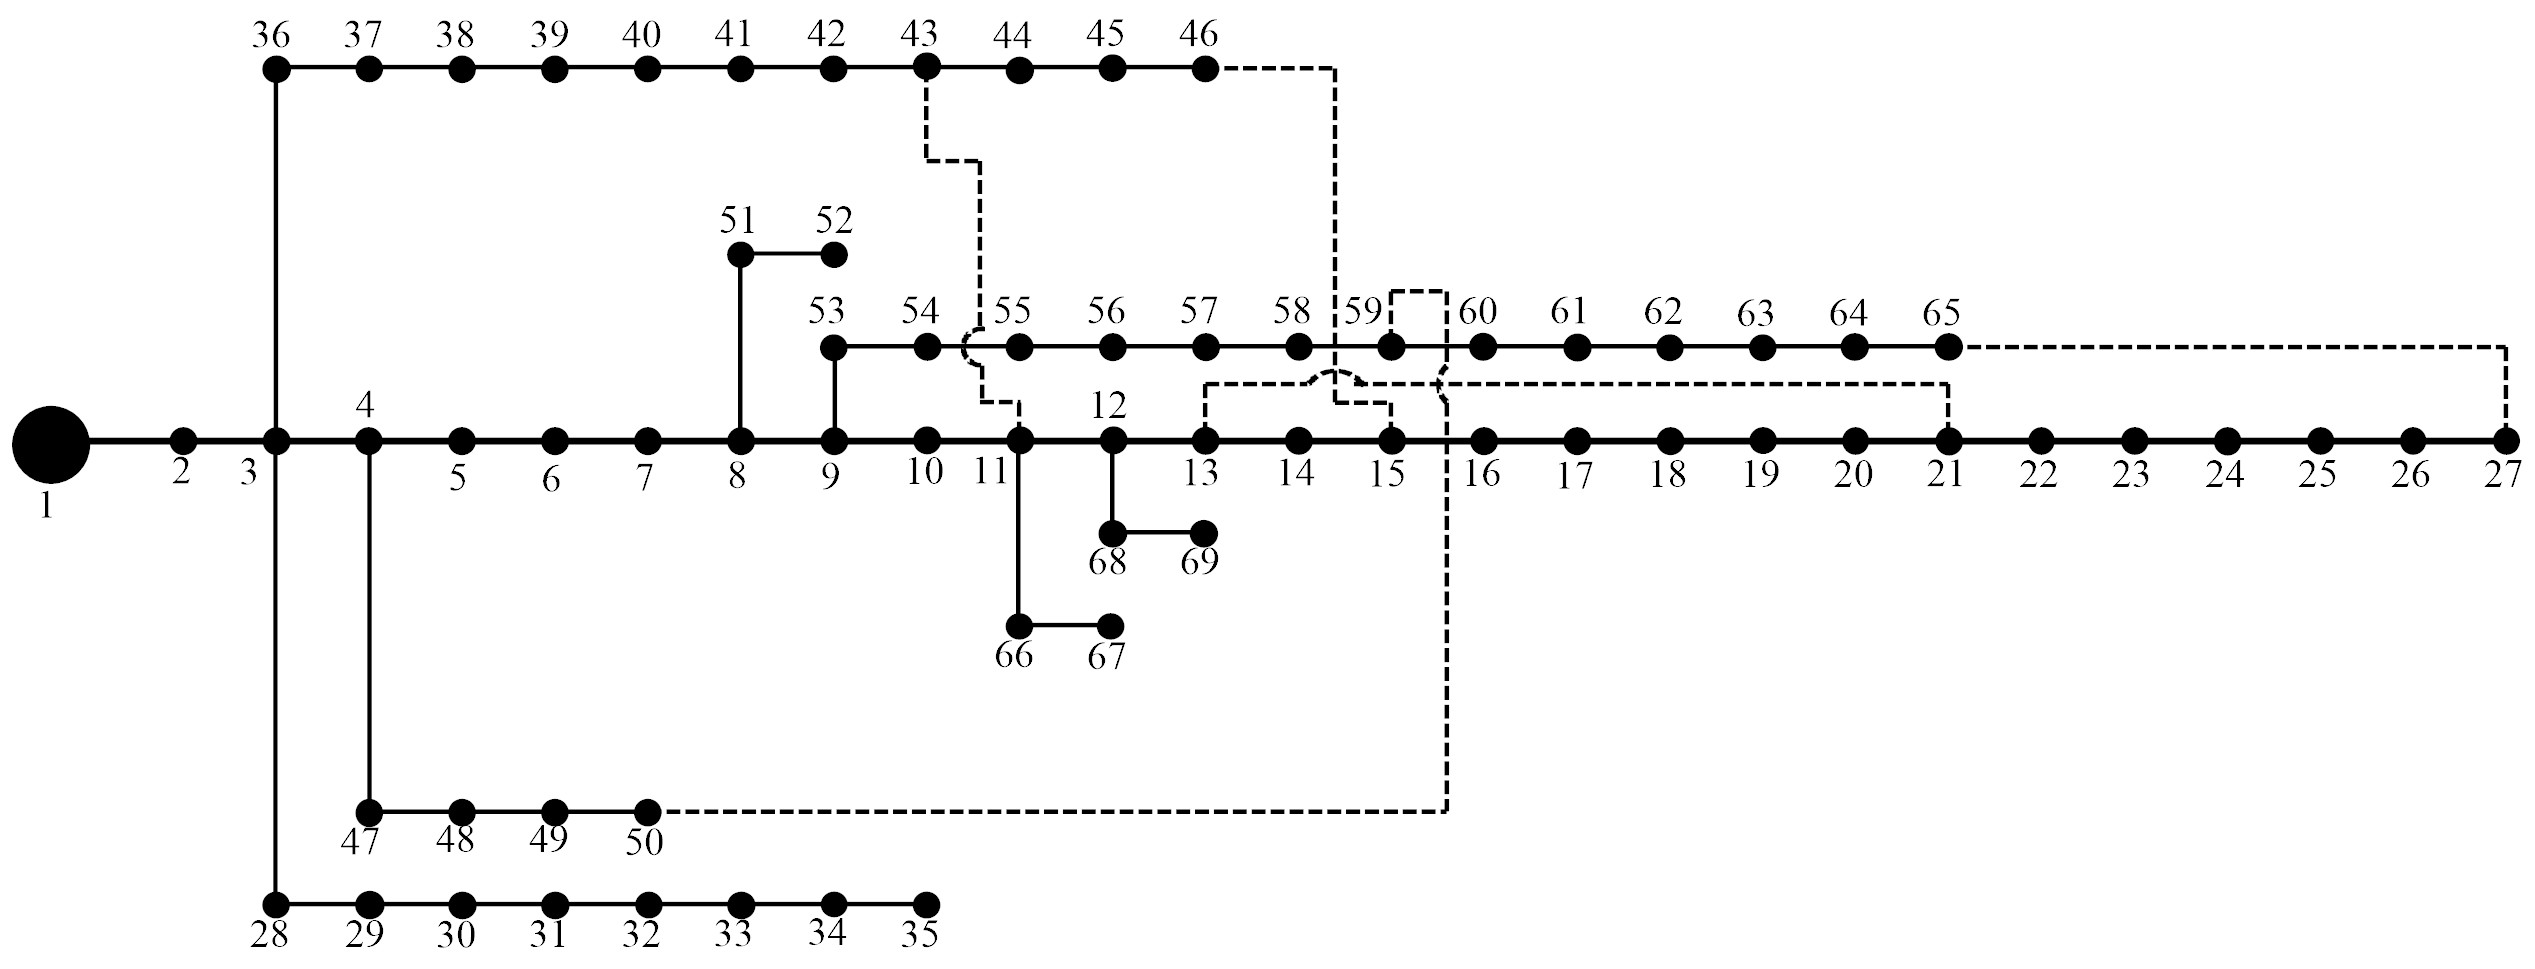
\includegraphics[width=1\textwidth]{./Figures/69bus_singleline_diagram_tieline_t1}
	\caption{Single line diagram of IEEE-69 Bus System}
	\label{fig:single69}
\end{figure}
\pagebreak
\begin{longtable}{cccccccccc}
	\caption {IEEE 69 Bus System Bus Data}
	\label{table:busdata69}
	\hline
	\multirow{3}{*}{\begin{tabular}[c]{@{}c@{}}Bus \\ No.\end{tabular}} & \multirow{3}{*}{\begin{tabular}[c]{@{}c@{}}Bus \\ Code\end{tabular}} & \multirow{3}{*}{\begin{tabular}[c]{@{}c@{}}Load\\ Type\end{tabular}} & \multicolumn{2}{c}{Load} & \multicolumn{4}{c}{Generator} & \multirow{2}{*}{\begin{tabular}[c]{@{}c@{}}Injected \\ MVAr\end{tabular}} \\  
	\cmidrule{4-5} 
	\cmidrule(lr{1em}){6-9}		 
	&  &  & \multicolumn{1}{l}{\multirow{2}{*}{MW}} & \multicolumn{1}{l}{\multirow{2}{*}{MVAr}} & \multicolumn{1}{l}{\multirow{2}{*}{MW}} & \multicolumn{1}{l}{\multirow{2}{*}{MVAr}} & \multicolumn{1}{l}{\multirow{2}{*}{Qmin}} & \multicolumn{1}{l}{\multirow{2}{*}{Qmax}} &  \\ 
	&  &  & \multicolumn{1}{l}{} & \multicolumn{1}{l}{} & \multicolumn{1}{l}{} & \multicolumn{1}{l}{} & \multicolumn{1}{l}{} & \multicolumn{1}{l}{} &  \\
	\cmidrule(lr){1-10}
	1 & 1 & - & 0 & 0 & 0 & 0 & 0 & 0 & 0 \\
	2 & 0 & Curtailable & 0 & 0 & 0 & 0 & 0 & 0 & 0 \\
	3 & 0 & Curtailable & 0 & 0 & 0 & 0 & 0 & 0 & 0 \\
	4 & 0 & Curtailable & 0 & 0 & 0 & 0 & 0 & 0 & 0 \\
	5 & 0 & Curtailable & 0 & 0 & 0 & 0 & 0 & 0 & 0 \\
	6 & 0 & Fixed & 0.0026 & 0.0022 & 0 & 0 & 0 & 0 & 0 \\
	7 & 0 & Controllable & 0.0404 & 0.0030 & 0 & 0 & 0 & 0 & 0 \\
	8 & 0 & Fixed & 0.0750 & 0.0054 & 0 & 0 & 0 & 0 & 0 \\
	9 & 0 & Fixed & 0.0300 & 0.0022 & 0 & 0 & 0 & 0 & 0 \\
	10 & 0 & Fixed & 0.0280 & 0.0019 & 0 & 0 & 0 & 0 & 0 \\
	11 & 0 & Fixed & 0.1450 & 0.1040& 0 & 0 & 0 & 0 & 0 \\
	12 & 0 & Fixed & 0.1450 & 0.1040 & 0 & 0 & 0 & 0 & 0 \\
	13 & 0 & Controllable & 0.0080 & 0.0055 & 0 & 0 & 0 & 0 & 0 \\
	14 & 0 & Controllable & 0.0080 & 0.0055 & 0 & 0 & 0 & 0 & 0 \\
	15 & 0 & Controllable & 0 & 0 & 0 & 0 & 0 & 0 & 0 \\
	16 & 0 & Controllable & 0.0455 & 0.0030 & 0 & 0 & 0 & 0 & 0 \\
	17 & 0 & Controllable & 0.0600 & 0.0350 & 0 & 0 & 0 & 0 & 0 \\
	18 & 0 & Controllable & 0.0600 & 0.0350 & 0 & 0 & 0 & 0 & 0 \\
	19 & 0 & Controllable & 0 & 0 & 0 & 0 & 0 & 0 & 0 \\
	20 & 0 & Controllable & 0.0010 & 0.0006 & 0 & 0 & 0 & 0 & 0 \\
	21 & 0 & Controllable & 0.1140 & 0.0810 & 0 & 0 & 0 & 0 & 0 \\
	22 & 0 & Controllable & 0.0530 & 0.0035 & 0 & 0 & 0 & 0 & 0 \\
	23 & 0 & Controllable & 0 & 0 & 0 & 0 & 0 & 0 & 0 \\
	24 & 0 & Controllable & 0.0280 & 0.020 & 0 & 0 & 0 & 0 & 0 \\
	25 & 0 & Controllable & 0 & 0 & 0 & 0 & 0 & 0 & 0 \\
	26 & 0 & Controllable & 0.0140 & 0.0100 & 0 & 0 & 0 & 0 & 0 \\
	27 & 0 & Curtailable & 0.0140 & 0.0100 & 0 & 0 & 0 & 0 & 0 \\
	28 & 0 & Curtailable & 0.0260 & 0.0186 & 0 & 0 & 0 & 0 & 0 \\
	29 & 0 & Curtailable & 0.0260 & 0.0186 & 0 & 0 & 0 & 0 & 0 \\
	30 & 0 & Curtailable & 0 & 0 & 0 & 0 & 0 & 0 & 0 \\
	31 & 0 & Curtailable & 0 & 0 & 0 & 0 & 0 & 0 & 0 \\
	32 & 0 & Curtailable & 0 & 0 & 0 & 0 & 0 & 0 & 0 \\
	33 & 0 & Curtailable & 0.0140 & 0.0100 & 0 & 0 & 0 & 0 & 0 \\
%	\toprule  \\ 
%	\toprule 
	34 & 0 & Curtailable & 0.0195 & 0.0140 & 0 & 0 & 0 & 0 & 0 \\
	35 & 0 & Controllable & 0.0060 & 0.0040 & 0 & 0 & 0 & 0 & 0 \\
	36 & 0 & Controllable & 0.0260 & 0.01855 & 0 & 0 & 0 & 0 & 0 \\
	37 & 0 & Controllable & 0.026 & 0.01855 & 0 & 0 & 0 & 0 & 0 \\
	38 & 0 & Controllable & 0 & 0 & 0 & 0 & 0 & 0 & 0 \\
	39 & 0 & Controllable & 0.0240 & 0.0170 & 0 & 0 & 0 & 0 & 0 \\
	40 & 0 & Controllable & 0.0240 & 0.0170 & 0 & 0 & 0 & 0 & 0 \\
	41 & 0 & Controllable & 0.0012 & 0.0100 & 0 & 0 & 0 & 0 & 0 \\
	42 & 0 & Controllable & 0 & 0 & 0 & 0 & 0 & 0 & 0 \\
		\toprule  \\ 
		\toprule 
	43 & 0 & Controllable & 0.0060 & 0.0043 & 0 & 0 & 0 & 0 & 0 \\
	44 & 0 & Controllable & 0 & 0 & 0 & 0 & 0 & 0 & 0 \\
	45 & 0 & Controllable & 0.03922 & 0.05263 & 0 & 0 & 0 & 0 & 0 \\
	46 & 0 & Controllable & 0.03922 & 0.0263 & 0 & 0 & 0 & 0 & 0 \\
	47 & 0 & Controllable & 0 & 0 & 0 & 0 & 0 & 0 & 0 \\
	48 & 0 & Controllable & 0.0790 & 0.0564 & 0 & 0 & 0 & 0 & 0 \\
	49 & 0 & Curtailable & 0.3847 & 0.2745 & 0 & 0 & 0 & 0 & 0 \\
	50 & 0 & Controllable & 0.3847 & 0.2745 & 0 & 0 & 0 & 0 & 0 \\
	51 & 0 & Curtailable & 0.0405 & 0.0283 & 0 & 0 & 0 & 0 & 0 \\
	52 & 0 & Curtailable & 0.0036 & 0.0027 & 0 & 0 & 0 & 0 & 0 \\
	53 & 0 & Curtailable & 0.00435 & 0.0035 & 0 & 0 & 0 & 0 & 0 \\
	54 & 0 & Curtailable & 0.0264 & 0.0190 & 0 & 0 & 0 & 0 & 0 \\
	55 & 0 & Curtailable & 0.0240 & 0.0172 & 0 & 0 & 0 & 0 & 0 \\
	56 & 0 & Curtailable & 0 & 0 & 0 & 0 & 0 & 0 & 0 \\
	57 & 0 & Fixed & 0 & 0 & 0 & 0 & 0 & 0 & 0 \\
	58 & 0 & Fixed & 0 & 0 & 0 & 0 & 0 & 0 & 0 \\
	59 & 0 & Fixed & 0.1000 & 0.0720 & 0 & 0 & 0 & 0 & 0 \\
	60 & 0 & Fixed & 0 & 0 & 0 & 0 & 0 & 0 & 0 \\
	61 & 0 & Controllable & 1.2440 & 0.8880 & 0 & 0 & 0 & 0 & 0 \\
	62 & 0 & Fixed & 0.0320 & 0.0230 & 0 & 0 & 0 & 0 & 0 \\
	63 & 0 & Fixed & 0 & 0 & 0 & 0 & 0 & 0 & 0 \\
	64 & 0 & Fixed & 0.2270 & 0.1620 & 0 & 0 & 0 & 0 & 0 \\
	65 & 0 & Fixed & 0.0590 & 0.0420 & 0 & 0 & 0 & 0 & 0 \\
	66 & 0 & Fixed & 0.0180 & 0.0130 & 0 & 0 & 0 & 0 & 0 \\
	67 & 0 & Fixed & 0.0180 & 0.0130 & 0 & 0 & 0 & 0 & 0 \\
	68 & 0 & Fixed & 0.0280 & 0.0200 & 0 & 0 & 0 & 0 & 0 \\
	69 & 0 & Controllable & 0.02800 & 0.0200 & 0 & 0 & 0 & 0 & 0 \\
	\bottomrule %[1.5pt]		
\end{longtable}
\flushleft
\item  Bus Code
\newline 1 - Slack Bus \newline 0 - Load Bus

\begin{longtable}{ccccccccc}
	\caption {IEEE 69 Bus System Line Data}
	\label{table:linedata69}
	\hline
	\multirow{4}{*}{\begin{tabular}[c]{@{}c@{}}  Line \\ No.\end{tabular}} & \multirow{4}{*}{\begin{tabular}[c]{@{}c@{}}From\\ Bus\end{tabular}} & \multirow{4}{*}{\begin{tabular}[c]{@{}c@{}}To\\ Bus\end{tabular}} & \multirow{4}{*}{\begin{tabular}[c]{@{}c@{}}R \\ (p.u)\end{tabular}} & \multirow{4}{*}{\begin{tabular}[c]{@{}c@{}}X\\ (p.u)\end{tabular}} & \multirow{4}{*}{\begin{tabular}[c]{@{}c@{}}B\\ (p.u)\end{tabular}} & \multirow{4}{*}{\begin{tabular}[c]{@{}c@{}}line code = 1\\ for lines\\ \textgreater{} 1 or \textless 1 for tr.tap\end{tabular}} & \multirow{4}{*}{\begin{tabular}[c]{@{}c@{}}Failure\\ Rate\\ (f/yr)\end{tabular}} & \multirow{4}{*}{\begin{tabular}[c]{@{}c@{}}Repair\\ Time\\ (h)\end{tabular}} \\
	
	&  &  &  &  &  &  &  &  \\
	&  &  &  &  &  &  &  &  \\
	&  &  &  &  &  &  &  &  \\
	\cmidrule{1-9} 
	1 & 1 & 2 & 0.0005 & 0.0012 & 0 & 1 & 0.0003 & 0.5 \\
	2 & 2 & 3 & 0.0005 & 0.0012 & 0 & 1 & 0.0003 & 0.5 \\
	3 & 3 & 4 & 0.0015 & 0.0036 & 0 & 1 & 0.0009 & 0.5 \\
	4 & 4 & 5 & 0.0251 & 0.0294 & 0 & 1 & 0.0156 & 0.5 \\
	5 & 5 & 6 & 0.3660 & 0.1864 & 0 & 1 & 0.2269 & 0.5 \\
	6 & 6 & 7 & 0.3811 & 0.1941 & 0 & 1 & 0.2363 & 0.5 \\
			\toprule  \\ 
	\toprule 
	7 & 7 & 8 & 0.0922 & 0.0470 & 0 & 1 & 0.0572 & 0.5 \\

	8 & 8 & 9 & 0.0493 & 0.0251 & 0 & 1 & 0.0306 & 0.5 \\
	
	9 & 9 & 10 & 0.8190 & 0.2707 & 0 & 1 & 0.5078 & 0.5 \\
	10 & 10 & 11 & 0.1872 & 0.0619 & 0 & 1 & 0.1161 & 0.5 \\
	11 & 11 & 12 & 0.7114 & 0.2351 & 0 & 1 & 0.4411 & 0.5 \\
	12 & 12 & 13 & 1.0300 & 0.3400 & 0 & 1 & 0.6386 & 0.5 \\
	13 & 13 & 14 & 1.0440 & 0.3450 & 0 & 1 & 0.6473 & 0.5 \\
	14 & 14 & 15 & 1.0580 & 0.3496 & 0 & 1 & 0.6560 & 0.5 \\
	15 & 15 & 16 & 0.1966 & 0.0650 & 0 & 1 & 0.1219 & 0.5 \\
	16 & 16 & 17 & 0.3744 & 0.1238 & 0 & 1 & 0.2321 & 0.5 \\
	17 & 17 & 18 & 0.0047 & 0.0016 & 0 & 1 & 0.0029 & 0.5 \\
	18 & 18 & 19 & 0.3276 & 0.1083 & 0 & 1 & 0.2031 & 0.5 \\
	19 & 19 & 20 & 0.2106 & 0.0690 & 0 & 1 & 0.1306 & 0.5 \\
	20 & 20 & 21 & 0.3416 & 0.1129 & 0 & 1 & 0.2118 & 0.5 \\
	21 & 21 & 22 & 0.0140 & 0.0046 & 0 & 1 & 0.0087 & 0.5 \\
	22 & 22 & 23 & 0.1591 & 0.0526 & 0 & 1 & 0.0986 & 0.5 \\
	23 & 23 & 24 & 0.3463 & 0.1145 & 0 & 1 & 0.2147 & 0.5 \\
	24 & 24 & 25 & 0.7488 & 0.2745 & 0 & 1 & 0.4643 & 0.5 \\
	25 & 25 & 26 & 0.3089 & 0.1021 & 0 & 1 & 0.1915 & 0.5 \\
	26 & 26 & 27 & 0.1732 & 0.0572 & 0 & 1 & 0.1074 & 0.5 \\
	27 & 3 & 28 & 0.0044 & 0.0108 & 0 & 1 & 0.0027 & 1.0 \\
	28 & 28 & 29 & 0.0640 & 0.1565 & 0 & 1 & 0.0397 & 1.0 \\
%	\toprule \\
%	\hline
	29 & 29 & 30 & 0.3978 & 0.1315 & 0 & 1 & 0.2466 & 1.0 \\
	30 & 30 & 31 & 0.0702 & 0.0232 & 0 & 1 & 0.0435 & 1.0 \\
	31 & 31 & 32 & 0.3510 & 0.1160 & 0 & 1 & 0.2176 & 1.0 \\
	32 & 32 & 33 & 0.8390 & 0.2816 & 0 & 1 & 0.5202 & 1.0 \\
	33 & 33 & 34 & 1.7080 & 0.5646 & 0 & 1 & 1.0590 & 1.0 \\
	34 & 34 & 35 & 1.4740 & 0.4873 & 0 & 1 & 0.9139 & 1.0 \\
	35 & 3 & 36 & 0.0044 & 0.0108 & 0 & 1 & 0.0270 & 1.0 \\
	36 & 36 & 37 & 0.0640 & 0.1565 & 0 & 1 & 0.0397 & 1.0 \\
	37 & 37 & 38 & 0.1053 & 0.1230 & 0 & 1 & 0.0653 & 1.0 \\
	38 & 38 & 39 & 0.0304 & 0.0355 & 0 & 1 & 0.0188 & 1.0\\
	39 & 39 & 40 & 0.0018 & 0.0021 & 0 & 1 & 0.0011 & 1.0 \\
	40 & 40 & 41 & 0.7283 & 0.8509 & 0 & 1 & 0.4515 & 1.0 \\
	41 & 41 & 42 & 0.3100 & 0.3623 & 0 & 1 & 0.1922 & 1.0 \\
	42 & 42 & 43 & 0.0410 & 0.0478 & 0 & 1 & 0.0254 & 1.0 \\ 
	43 & 43 & 44 & 0.0092 & 0.0116 & 0 & 1 & 0.0057 & 1.0 \\
	44 & 44 & 45 & 0.1089 & 0.1373 & 0 & 1 & 0.0675 & 1.0 \\
	45 & 45 & 46 & 0.0009 & 0.0012 & 0 & 1 & 0.0006 & 1.0 \\
	46 & 4 & 47 & 0.0034 & 0.0084 & 0 & 1 & 0.0021 & 1.0 \\
	47 & 47 & 48 & 0.0851 & 0.2083 & 0 & 1 & 0.0528 & 1.0 \\
	48 & 48 & 49 & 0.2898 & 0.7091 & 0 & 1 & 0.1797 & 1.0 \\
	49 & 49 & 50 & 0.0822 & 0.2011 & 0 & 1 & 0.5100 & 1.0 \\
	50 & 8 & 51 & 0.0928 & 0.0473 & 0 & 1 & 0.0575 & 1.0 \\
	51 & 51 & 52 & 0.3319 & 0.1114 & 0 & 1 & 0.2058 & 1.0 \\
	52 & 9 & 53 & 0.1740 & 0.0886 & 0 & 1 & 0.1079 & 1.0 \\
			\toprule\\
	\hline
	53 & 53 & 54 & 0.2030 & 0.1034 & 0 & 1 & 0.1259 & 1.0 \\

	54 & 54 & 55 & 0.2842 & 0.1447 & 0 & 1 & 0.1762 & 1.0 \\
	55 & 55 & 56 & 0.2813 & 0.1433 & 0 & 1 & 0.1744 & 1.0 \\
	56 & 56 & 57 & 1.5900 & 0.5337 & 0 & 1 & 0.9858 & 1.0 \\
	57 & 57 & 58 & 0.7837 & 0.263 & 0 & 1 & 0.4859 & 1.0 \\
	58 & 58 & 59 & 0.3042 & 0.1006 & 0 & 1 & 0.1886 & 1.0 \\
	59 & 59 & 60 & 0.3861 & 0.1172 & 0 & 1 & 0.2394 & 1.0 \\
	60 & 60 & 61 & 0.5075 & 0.2585 & 0 & 1 & 0.3146 & 1.0 \\
	61 & 61 & 62 & 0.0974 & 0.0496 & 0 & 1 & 0.6040 & 1.0 \\
	62 & 62 & 63 & 0.1450 & 0.0738 & 0 & 1 & 0.0899 & 1.0 \\
	63 & 63 & 64 & 0.7105 & 0.3619 & 0 & 1 & 0.4405 & 1.0 \\
	64 & 64 & 65 & 1.0410 & 0.5302 & 0 & 1 & 0.6454 & 1.0 \\
	65 & 11 & 66 & 0.2012 & 0.0611 & 0 & 1 & 0.1247 & 1.0 \\
%	\toprule\\
%	\hline
	66 & 66 & 67 & 0.0047 & 0.0014 & 0 & 1 & 0.0029 & 1.0 \\
	67 & 12 & 68 & 0.7394 & 0.2444 & 0 & 1 & 0.4584 & 1.0 \\
	68 & 68 & 69 & 0.0047 & 0.0016 & 0 & 1 & 0.0029 & 1.0 \\
	69* & 11 & 43 & 0.5000 & 0.5000 & 0 & 1 & 0.3100 & 1.0 \\
	70* & 13 & 21 & 0.5000 & 0.5000 & 0 & 1 & 0.3100 & 1.0 \\
	71* & 15 & 46 & 1.0000 & 1.0000 & 0 & 1 & 0.6200 & 1.0 \\
	72* & 50 & 59 & 2.0000 & 2.0000 & 0 & 1 & 1.2100 & 1.0 \\
	73* & 27 & 65 & 1.0000& 1.0000 & 0 & 1 & 0.6200 & 1.0 \\
	\bottomrule
\end{longtable}
\newline *- Tie Line	
	

%\end{document}